\section{Entropie}

\subsection{Begrip Entropie}

Onze Kelvinschaal is zo gekozen zodat:
\[
\frac{T}{T'} = \frac{Q}{Q'} = \frac{\phi(T_e)}{\phi(T'_e)}
\]

Waardoor \(T = k \phi (T_e)\) met k een arbitraire constante... Of toch niet? 

Herinner u de warmte-overdracht van twee nabij gelegen RA-oppervlakken?
\[
\dbar Q = \phi (T_e) f(\sigma) d\sigma
\]
\[
\implies \dbar Q = \frac{T}{k} f(\sigma) d\sigma 
\]
\[\implies \frac{\dbar Q}{T} = \frac{1}{k} f(\sigma) d\sigma \]

Nu is het rechterlid een differentiaal van een functie van de toestand, namelijk \(S\), die we \textbf{entropie} noemen.
\[ \frac{\dbar Q_{rev}}{T} = dS\]

Bij een eindige verandering van toestand kunnen we dit integreren:
\[\int_{i}^{f} \frac{\dbar Q_{rev}}{T} = \int_{i}^{f} dS = S_f - S_i\]

Absolute entropie is niet gedefinieerd, maar veranderingen in entropie wel. We kunnen dus enkel \(\Delta S\) bepalen, niet \(S\) zelf.

Voor een reversibel proces geldt:
\[d S = \oint_{\text{reversibel}}
 \frac{\dbar Q_{rev}}{T} = 0\]

 Dit is het Clausius-theorema dat werd afgeleid uit de Carnot-cyclus.

\subsection{Entropie Ideaal Gas}

Herinner u voor een ideaal gas is de eerste hoofdwet:
\[\dbar Q = C_P dT - P dV\]
\[\implies \frac{\dbar Q}{T} = \frac{C_P}{T} dT - \frac{P}{T} dV\]
\[\implies \Delta S = \int_{T_1}^{T} \frac{C_P}{T} dT - \int_{V_1}^{V} \frac{P}{T} dV\]
Als \(C_P = cst\):
\[ S-S_1 = C_P \ln \left(\frac{T}{T_1}\right) - nR \ln \left(\frac{V}{V_1}\right)\]
\[S = C_P \ln T-nR \ln V -C_P \ln T_1 + nR\ln V_1 + S_1 = C_P\ln T-nR\ln V +S_0 \]

\[\boxed{S = C_P\ln T-nR\ln V + S_0} \qquad (C_P = cst)\]


Ook geldt:
\[\dbar Q = C_V dT + P dV\]

\[S = \int_{T_1}^{T} \frac{C_V}{T} dT + nR \int_{V_1}^{V} \frac{dV}{V}\]

Als \(C_V = cst\):
\[\boxed{S = C_V \ln T + nR \ln V + S_0} \qquad (C_V = cst)\]

\subsection{TS-Diagrammen}

Zoals we eerder al een wilde encounter hadden met een TS-diagram de Carnot-cyclus zullen we hier nu verder op ingaan.

\begin{figure}
    \centering
    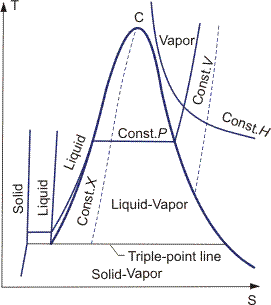
\includegraphics[width=0.8\textwidth]{Foto's-Figuren/TS-Diagram.png}
    \caption{TS-diagram \copyright{Muller-Steinhagen, Hans Michael Gottfried  DOI: 10.1615/AtoZ.t.thermodynamics}}
\end{figure}



\[
\dbar Q_R = TdS \implies Q_R = \int_{i}^{f} TdS
\]



\begin{definition}
    Een \textbf{Isentroop} proces is een reversibel adiabatisch proces, dus waarbij de entropie constant blijft, dus \(dS = 0\).
\end{definition}

De warmtecapaciteiten worden dan:
\[\left(\frac{\dbar Q}{dT}\right)_V = C_V = T\left(\frac{\partial S}{\partial T}\right)_V \qquad (\text{isentroop}, V=cst)\]
en 
\[\left(\frac{\dbar Q}{dT}\right)_P = C_P = T\left(\frac{\partial S}{\partial T}\right)_P \qquad (\text{isentroop}, P=cst)\]

Als \(C_P(T)\) en/of \(C_V(T)\) gekend zijn, kunnen we de entropieverandering van een ideaal gas bepalen:
\[S_f -S_i = \int_{T_1}^{T} \frac{C_V(T)}{T} dT   \qquad (rev, V = cst)\]
\[S_f-S_i = \int_{T_1}^{T} \frac{C_P(T)}{T} dT  \qquad (rev, P = cst)\]

\subsection{De Carnot cyclus}

Misschien kunnen jullie zich de TS-diagram van figuur \ref{Fig:carnot-cycl} nog herinneren. 

\begin{definition}
    De Carnot-cyclus is een reversibele machine werkend tussen slechts twee warmtereservoirs.
\end{definition}

Een warmte-overdracht bij de Carnot-cyclus tussen twee RA-oppervlakken geeft:
\[\frac{Q_H}{T_H} = \frac{Q_K}{T_K}\]
\[\implies \frac{Q_H}{Q_K} = \frac{T_H}{T_K}\]
Waaruit het rendement:
\[\eta = 1 - \frac{Q_K}{Q_H} = 1 - \frac{T_K}{T_H}\] 

Dus
\[
\eta_{\text{Carnot}} = 1 - \frac{T_K}{T_H}
\]

Een rendement van 100\% is alleen mogelijk als \(T_K = 0\) K, wat onmogelijk is volgens de derde hoofdwet van de thermodynamica. Daarom is een rendement van 100\% onbereikbaar.

\begin{postulate}
    Voor elk reversibel proces blijft de entropie van het universum constant. 
\end{postulate}

\subsection{Entropie en Irreversibiliteit}

\begin{definition}[Irreversibel Proces]
    Een proces is irreversibel als het niet mogelijk is om het proces in omgekeerde richting te laten verlopen zonder veranderingen in de omgeving.
    Zo een proces kan beschreven worden als:
    \[\Delta S_{sys} = S_f-S_i = \int_{i, \text{Rev}}^{f} \frac{\dbar Q}{T}\]
    De integratie gebeurt hier langs een (vervangend) reversibel pad (maar niet langs het oorspronkelijke pad), maar het proces zelf is irreversibel.
\end{definition}

\subsubsection{Uitwendige Mechanische Irreversibiliteit}

De irreversibel verrichte arbeid kunnen we vervangen door een reversibel proces met reversibele isobare overdracht van warmte, zodat we de entropieverandering kunnen bepalen:
\[\Delta S_{sys} = \int_{T_i, \text{Rev}}^{T_f} \frac{\dbar Q}{T} = \int_{T_i, \text{Rev}}^{T_f} C_P\frac{dT}{T}\]
Als \(C_P\) constant is:
\[\Delta S_{sys} = C_P \ln \left(\frac{T_f}{T_i}\right) \qquad (C_P = cst)\]


\subsubsection{Interne Mechanische Irreversibiliteit}

Vb: een isotherm proces van een ideaal gas met dus \(\dbar Q_R = PdV\)
\[\implies \frac{\dbar Q_R}{T} = nR\frac{dV}{V}\]

Entropieverandering:
\[\Delta S_{sys} = \int_{Rev,V_i}^{V_f} nR\frac{dV}{V} = nR \ln \left(\frac{V_f}{V_i}\right)\]

\subsubsection{Externe Thermische Irreversibiliteit}
\[\Delta S_{\text{univ}} = \sum \Delta S = \frac{Q}{T_K} - \frac{Q}{T_H}\]

\subsubsection{Chemisch Irreversibel Proces}

Vb: diffusie twee verschillende inerte gassen:

stel \(\frac{V_i}{n} = 1\) en \(\frac{V_f}{n} = 2\), dan is de entropieverandering:
\[\Delta S_{sys} =  R \ln \left(\frac{2}{1}\right) + R \ln \left(\frac{2}{1}\right) = 2R \ln 2\]

Niet zo een belangrijk voorbeeld denk ik \(\dots\)

\subsection{Entropietoename Universum}

Entropie in het universum neemt steeds toe (tot het concept tijd niet meer bestaat \(\dots\))

\begin{proof}[Entropieprincipe]
    Het is voldoende ons te beperken tot adiabatische processen.

    We starten in ons systeem met coördinaten \(T, X\) en \(X'\) op punt \(i\) en eindigen op punt \(f\). 
    We kunnen nu een irreversibel pad vinden van \(i \to f\): 
    \[
    \Delta S = S_f - S_i 
    \]
    en een irreversibel adiabatisch proces van \(f \to k\) zodat de temperatuur \(T'\) wordt van een willekeurig gekozen reservoir.

    Het systeem wordt nu in contact gebracht met dit reservoir, er wordt een reviersibel isotherm proces van \(k \to j\) tot ze dezelfde entropie hebben als in punt \(i\).

    Nu gaan we van dit punt terug \(j\) terug naar \(i\) via een reversibel adiabatisch proces.

    De twee processen \(i \to f\) en \(j \to k\) brengen een entropoieverandering met zich mee, en de nette entropieverandering van een cyclus is \(0\), dus:

    \[
    (S_f-S_i) + (S_j- S_k) = \Delta S + S_j - S_k = 0
     \implies \Delta S = S_k - S_j
    \]
    De enige warmte-overdracht gebeurt tussen \(k\) en \(j\), en aangezien \(T' > T\) (omdat \(T'\) van een reservoir is), zal er warmte van \(k \to j\) stromen:

    \[
    Q_R = T' (S_j-S_k)
    \]

    De hoeveelheid arbeid verricht is:

    \[
    W_{net} = Q_R
    \]

    Volgens de tweede wet kan kan er geen warmte in het systeem gebracht zijn.
    \footnote{Anders zouden we een machine hebben die werkt tussen een reservoir en een systeem, en die alleen warmte onttrekt aan het reservoir en arbeid levert, wat onmogelijk is volgens de tweede wet.}

    Dus \(Q_R<0\):

    \[
    T' = (S_j-S_k) \leq 0 
    \]
    \[
    \implies \Delta S = S_k - S_j \geq 0
    \]

    We kunnen nu veronderstellen dat ons eerste irreversibel adiabatisch proces van \(i \to f\) zou verlopen zonder dat er een entropieverandering zou optreden, dus \(\Delta S = 0\).
    Doordat \(\implies \Delta Q = 0 \), dan zal ook \(W_{net} = 0\) en is er geen toestandsverandering (systeem is terug in punt \(i\)).
    Maar dit betekend dat het proces reversibel is, wat in tegenspraak is met onze aanname dat het proces irreversibel is.

    Dus de entropieverandering kan niet nul zijn, en moet dus positief zijn.

    \qed
\end{proof}

\begin{postulate}
    De entropieverandeiring van een systeem en zijn omgeving is altijd positief en nadert slechts naar 0 als de processen naar reversibiliteit naderen.